\PassOptionsToPackage{dvipsnames}{xcolor}


\documentclass{article}


\usepackage[left=3cm,right=3cm,top=2cm,bottom=3cm]{geometry} % page settings
\usepackage{amsmath,amsfonts,amsthm,amssymb} % provides many mathematical environments & tools
 
 \usepackage{examplep}


\usepackage{tikz}
\usetikzlibrary{shapes,arrows,positioning}
\usetikzlibrary{mindmap,trees, backgrounds}
\usetikzlibrary{decorations.pathreplacing}
\usetikzlibrary{calc}

%\usepackage[dvipsnames]{xcolor}

%\tikzset{block/.style={rectangle, draw, text width=10em, text centered, rounded corners,
 %minimum width=3.5cm}}
 %\tikzset{blockL/.style={rectangle, draw, text width=14em, text centered, rounded corners,
 %minimum width=3.5cm}}
%\tikzset{block_color/.style={rectangle, draw, fill=BurntOrange!65, text width=10em, text centered, rounded corners,
 %minimum width=3.5cm}}
 %\tikzset{line/.style={draw, -latex}}
 
 %\definecolor{green_m}{rgb}{0.0, 0.66, 0.47}
 
 
%\usepackage{adjustbox}

\usepackage{bigints}
\usepackage{hyperref}
%\newcommand{\lver}{\left|}
%\newcommand{\rver}{\right|}
%\newcommand{\bsy}[1]{\boldsymbol{#1}}

\usepackage{hyperref}
\hypersetup{%
  colorlinks=false,% hyperlinks will be black
  linkbordercolor=black,% hyperlink borders will be red
  pdfborderstyle={/S/U/W 1}% border style will be underline of width 1pt
}


% hyperref
\usepackage[]{hyperref}

% color box
%\newcommand{\boxcolor}{orange}
\makeatletter
%\renewcommand{\boxed}[2]{\textcolor{#2}{%
%\tikz[baseline={([yshift=-1ex]current bounding box.center)}] \node [thick, rectangle, minimum width=1ex,rounded corners,draw] {\normalcolor\m@th$\displaystyle#1$};}}



 \makeatother
\begin{document}

\title{Deep Learning Mini-Project 2 Report \\ Implementing from Scratch a Mini Deep-Learning Framework.}
\author{Group 78\footnote{As agreed with Dr. F. Fleuret, L. Pegolotti has collaborated with group 78 for Project 1 and with group 79, with M. Martin, for Project 2. C. Bigoni and N. Ripamonti have worked together on both projects.}  \\ Caterina Bigoni and Nicol\`o Ripamonti}
\date{18 May 2018}
\maketitle
%\tableofcontents
%\newpage



% \small{\textsuperscript{a}EPFL-SB-MATH-MCSS, \textsuperscript{b}EPFL-SB-MATH-DIV}


\section{Introduction}
The goal of this project consists in designing a mini deep learning network frameworks ``by scratch''. 
We have therefore built a network that combines fully connected layers, Tanh, the logistic sigmoid and ReLu. 
Moreover, we have implemented a forward and backward pass as well as the update of parameters using the stochastic gradient descent (SGD).
For this part we followed the mathematical framework described in the lecture notes. 

This report is organised as follows: in Section \ref{sec_code} we describe the generalities of the implementation, explaining in particular the concept of dictionaries used to define the operators and their connectivity map. 
Then, in  Section \ref{sec_numexp}, we test the constructed network on a two-class classification problem both for a linearly separable dataset and a non-linearly separable one.
Satisfactory results, i.e. from 0.5 to 2\% error, are achieved in both cases. 
Conclusions and further remarks are presented in Section \ref{sec_conclusion}.

\section{General Network}\label{sec_code}
The library handles the network structure by means of dictionaries, the ideal type to represent graphs in Python language . 
The generic dictionary considered for this project can be written as
\begin{align*}
\PVerb{Dictionary} =  \{  & \text{ key}_1  \: : [ \text{ value}_{1,1},  \text{ value}_{1,2}, \dots] ,  \\
&  \text{ key}_2  \: : [ \text{ value}_{2,1},  \text{ value}_{2,2},  \dots] , \\
& \dots \\
& \text{ key}_N  \: : [ \text{ value}_{N,1},  \text{ value}_{N,2},  \dots]  \},
\end{align*}
where for each key we may have an arbitrary (and possibly different) number of values. 
We use the list constructor $[ \dots ]$ to gather all the values related to a certain key because lists are containers easily iterable and we need this feature as explained later on. \\
The first dictionary that the user has to define is called \verb|operators| in \verb|test.py| and it records the modules used in the network. 
For example, let us consider a simple network, as the one represented in Figure \ref{example_graph}.
Its related dictionary is
\begin{align*}
\PVerb{operators} =  \{  & 1  \: :  \text{ Linear1 }, \: 2  \: : \text{ Nonlinear1 },\\
&  3  \: :  \text{ Linear2 }, \: 4  \: :  \text{ Nonlinear2 },\\
&  5  \: :  \text{ Sum }, \: 6 \: : \text{ Linear3 } \}.
\end{align*}
%\begin{align*}
%\text{operators} =  \{  & 1  \: :  \text{ Linear1 }  , \: 2  \: : \text{ Nonlinear1 }   , \\
%&  3  \: :  \text{ Linear2 }   , \: 4  \: : \text{ Nonlinear2 }  , \} \\
%&   5  \: :  \text{ Sum }   , 1  \: :  \text{ Linear3 }  \}.\\ 
%\end{align*}
The next step is the definition of a \verb|connectivity| dictionary: the rationale behind this dictionary is to describe the relations between each module and its followings in the natural ordering of the network from the inputs to the output. In this interpretation of Python dictionary, a key represents the module we are considering in a certain moment and the related values are other modules waiting for its output. Then \verb|operators| dictionary is used to translate numerical values to proper modules.The \verb|connectivity| matrix of the considered example would then be
\begin{align*}
\PVerb{connectivity} =  \{  & 1  \: :  [ \: 2 \: ], \: 2  \: : [ \: 5 \: ],\\
&  3  \: :  [ \: 4 \: ], \: 4  \: :  [ \: 5 \: ],\\
&  5  \: :  [ \: 6 \: ]  \}.
\end{align*}
During the initialization of \verb|Network| object, the \verb|connectivity| matrix is translated into two additional dictionaries that are more useful for the forward and backward passes. Consider the forward pass first: the idea is that, given a certain module, we have to know the outputs of the previous modules in the graph, the exact opposite of what is offered by \verb|connectivity|. Hence, after storing the necessary data, the constructor of \verb|Network| generates the dictionary \verb|connectivity_forward|. In the test case we have
\begin{align*}
\PVerb{connectivity_forward} =  \{  & 2  \: :  [ \: 1 \: ], \: 4  \: : [ \: 3 \: ],\\
&  5  \: :  [ \: 2 , 4 \: ], \: 5  \: :  [ \: 6 ] \}.
\end{align*} 
After \verb|Python 3.60|, looping over a dictionary is done in the order in which the dictionary is defined but, to avoid unexpected behaviour with previous releases, we force this property by using the \verb|OrderedDict| container provided by the \verb|Python| module \verb|collections|.
While the structure of \verb|connectivity| might work for the backpropagation of the gradients, we need to reverse the order and  obtain
\begin{align*}
\PVerb{connectivity_backward} =  \{  & 5  \: :  [ \: 6 \: ], 4  \: : [ \: 5 \: ],\\
&  2  \: :  [ \: 5 \: ], 1  \: :  [ \: 2 \: ],\\
&  3  \: :  [ \: 4 \: ]  \}.
\end{align*}
\begin{figure}[h]
 \begin{center}
  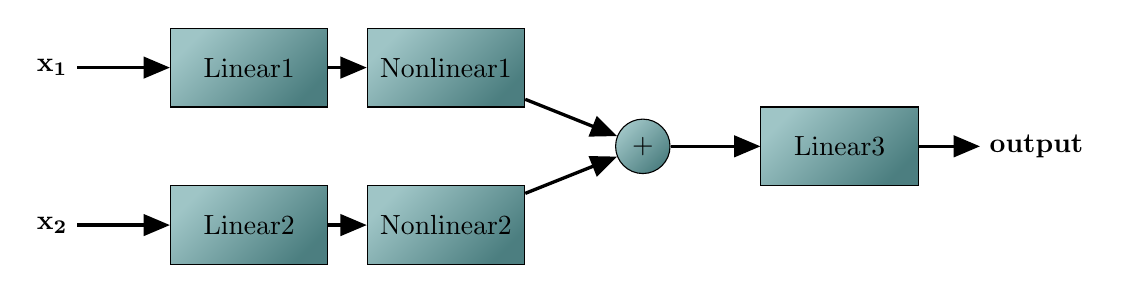
\begin{tikzpicture}
    %%Create a style for the arrows we are using
    \tikzset{normal arrow/.style={draw,-triangle 45,very thick}}
    %%Create the different coordinates to place the nodes
    \coordinate (1) at (0,0);
    \coordinate (2) at (2.5,0);
    \coordinate (3) at (2.5,-2);
    \coordinate (4) at (0,-2);
    \coordinate (5) at (5,-1);
    \coordinate (6) at (7.5,-1);
    \coordinate (x1) at (-2.5,0);
    \coordinate (x2) at (-2.5,-2);
    \coordinate (out) at (10,-1);
    %% Draw nodes
        \node[draw,rectangle,shading=axis,top color=CadetBlue!60, bottom color=CadetBlue!80!black,shading angle=45,minimum width = 2cm, minimum height = 1cm] (n1) at (1) {Linear1};
        \node[draw,rectangle,shading=axis,top color=CadetBlue!60, bottom color=CadetBlue!80!black,shading angle=45,minimum width = 2cm, minimum height = 1cm] (n2) at (2) {Nonlinear1};
        \node[draw,rectangle,shading=axis,top color=CadetBlue!60, bottom color=CadetBlue!80!black,shading angle=45,minimum width = 2cm, minimum height = 1cm] (n3) at (3) {Nonlinear2};
        \node[draw,rectangle,shading=axis,top color=CadetBlue!60, bottom color=CadetBlue!80!black,shading angle=45,minimum width = 2cm, minimum height = 1cm] (n4) at (4) {Linear2};
         \node[draw,circle,shading=axis,top color=CadetBlue!60, bottom color=CadetBlue!80!black,shading angle=45] (n5) at (5) {+}; 
         \node[draw,rectangle,shading=axis,top color=CadetBlue!60, bottom color=CadetBlue!80!black,shading angle=45,minimum width = 2cm, minimum height = 1cm] (n6) at (6) {Linear3};         
        \node (nx1) at (x1) {$\mathbf{x_1}$};
        \node (nx2) at (x2) {$\mathbf{x_2}$};
        \node (xout) at (out) {$\mathbf{output}$};
    %%Drawing the arrows
    \path[normal arrow] (nx1) -- (n1);
    \path[normal arrow] (nx2) -- (n4);
    \path[normal arrow] (n1) -- (n2);
    \path[normal arrow] (n4) -- (n3);
    \path[normal arrow] (n2) -- (n5);
    \path[normal arrow] (n3) -- (n5);
    \path[normal arrow] (n5) -- (n6);
    \path[normal arrow] (n6) -- (xout);
  \end{tikzpicture}
  \caption{Example of network that can be represented using our library. In the graph, $x_1$ and $x_2$ represent possible inputs.}
  \label{example_graph}
  \end{center}
\end{figure}  



% Modules
\subsection{Modules}
With the term \emph{module} we mean each possible element of the network from linear or nonlinear layers to the loss function. 
Moreover, other operators such as the sum of two different inputs are treated as modules, and hence we obtain an simpler representation for more complex networks.
The general structure of a module object is given in \verb|ModuleBase.py| and in each derived object we have to define the following methods:
\begin{itemize}
\item \verb|forward|: Implement the forward pass given the input of the module and store both the input and the output as attributes of the class. 
\item \verb|backward|: Compute the gradient of the loss with respect to the input given the gradient of the loss with respect to the output. If the module contains parameters, it also computes the gradient of the loss with respect to them.
\item \verb|update_param|: Given a learning rate as input, updates the parameters of the module using a gradient descent based approach.
\end{itemize}
The reason behind this structure is that the for the optimization phase we are using a gradient descent based method. Given a functional $\mathcal{L}:\mathbb{R}^D \mapsto \mathbb{R}$, and a starting point $\omega_0\in\mathbb{R}^D$, a local approximation of $\mathcal{L}$ allows to find a point 
\begin{equation*}
\omega = \omega_0 - \eta \nabla \mathcal{L}(\omega_0)
\end{equation*}
such that, if $\eta$ is small enough, $\mathcal{L}(\omega)<\mathcal{L}(\omega_0)$. \\
In our case $\omega$ represents the set of parameters related to each module and $\mathcal{L}$ a functional measuring the prediction error of the method. To use this in a neural network code we need to understand how the gradient of the loss $\mathcal{L}$ with respect to the parameters is computed. The action of a generic $\sigma$-parametrized module on an input signal $x^{l-1}$ to produce the output  $x^{l}$ can be written as
\begin{equation*}
x^{l} = f( x^{l-1} ; \sigma).
\end{equation*}
Thanks to the chain-rule of differentiation, we have
\begin{equation}\label{gradwrtparam}
\nabla_{\sigma} \mathcal{L} = \nabla_{x^l} \mathcal{L} \left ( \nabla_{\sigma} x^l \right )^T,
\end{equation}
where $\nabla_{\sigma} x^l$ depends on the specific function. Hence, $\nabla_{\sigma} \mathcal{L}$ can be computed if the module receives as input $\nabla_{x^l} \mathcal{L}$. \\
The next step consists in the backpropagation of the information regarding the derivative of the loss function with respect to the input, so that previous models can compute $\nabla_{\sigma} \mathcal{L}$. Using again the chain-rule for differentiation we get
\begin{equation}\label{gradwrtinput}
\nabla_{x^{l-1}}  \mathcal{L} = \left(  \nabla_{x^{l-1}}  x^{l} \right)^T  \nabla_{x^l} \mathcal{L}.
\end{equation}
If $f$ is a nonlinearity such that $x^l_i$ depends just on $x^{l-1}_i$, then $\nabla_{x^{l-1}} x^l$ is a diagonal matrix and (\ref{gradwrtinput}) is reduced to a pointwise multiplication and we exploit this in the code.
\subsubsection{Linear Layer}
In our code the linear layer, generically represented by the operation
\begin{equation*}
x^l = A x^{l-1} + b , 
\end{equation*}
with $x^{l-1}\in \mathbb{R}^{n_{inp}}, x^{l}\in \mathbb{R}^{n_{out}}, b\in \mathbb{R}^{n_{out}}, A\in \mathbb{R}^{n_{inp}\times n_{out}}$, is the only one containing parameters. Since gradient descent is implemented using a stochastic mini-batch approach, we adapted (\ref{gradwrtinput}) and (\ref{gradwrtparam}) to have a vectorized code. A common choice is to have the number of samples as first dimension of the input, hence each contribution of relations (\ref{gradwrtinput}) and (\ref{gradwrtparam}) has to be transpose. Particular attention has been paid to the update of $\nabla_{\sigma} \mathcal{L}$: suppose that we are considering batches of size $n_b$,  (\ref{gradwrtparam}) is given by
\begin{equation*}
\nabla_{A} \mathcal{L} =\left (\nabla_{x^l} \mathcal{L} \right )^T  X^{l-1} ,
\end{equation*}
with $X^{l-1}\in\mathbb{R}^{n_p \times n_{inp}}$. Since in this way in $\nabla_{A} \mathcal{L}$ we compute the sum of the gradients, we rescale by $n_p$ to have the average.
\subsubsection{Nonlinear Activation functions}
As previously mentioned, for nonlinear operators, equation (\ref{gradwrtinput}) is simplified to
\begin{equation*}
\nabla_{x^{l-1}}  \mathcal{L} = \text{diag} \left ( \nabla_{x^{l-1}}  x^{l} \right) \circ  \nabla_{x^l} \mathcal{L}.
\end{equation*}
We implemented 3 different types of nonlinear activation. 
\begin{itemize}
\item \underline{Rectified Linear Unit}:
\begin{equation*}
x^{l} = f(x^{l-1})
= 
\begin{cases}
&x^{l-1}, \quad \text{if } x^{l-1}>0, \\
&0, \quad \text{otherwise}.
\end{cases}
\qquad 
\text{diag} \left ( \nabla_{x^{l-1}}  x^{l} \right) = 
\begin{cases}
&1, \quad \text{if } x^{l-1}>0, \\
&0, \quad \text{otherwise},
\end{cases}
\end{equation*}
\item \underline{Logistic Sigmoid}:
\begin{equation*}
x^{l} = f(x^{l-1})
= 
\dfrac{1}{1-e^{-x^{l-1}}},
\qquad
\text{diag} \left ( \nabla_{x^{l-1}}  x^{l} \right) = 
f(x^{l-1})(1-f(x^{l-1})),
\end{equation*}
\item \underline{Hyperbolic Tangent}:
\begin{equation*}
x^{l} = f(x^{l-1})
= 
\text{tanh}(x^{l-1}),
\qquad
\text{diag} \left ( \nabla_{x^{l-1}}  x^{l} \right) = 
1-(\text{tanh}(x^{l-1}))^2,
\end{equation*}
\end{itemize}
\subsubsection{Sum operator}
The sum operator does not have any parameter and is simply described by
\begin{equation*}
x^{l} = x_1^{l-1} + x_2^{l-1} + \dots + x_N^{l-1}
\end{equation*}
Moreover,
\begin{equation*}
\text{diag} \left ( \nabla_{x_i^{l-1}}  x^{l} \right) = 1, \qquad i=1,\dots,N.
\end{equation*}
\section{Numerical Experiments}\label{sec_numexp}
% simple model on linear data
We run a simple ``sanity check'' test to verify if our setup behaves correctly.
We first consider a simpler classification problem: a two-class  problem where the discriminant line that separates  points classified with label 0 or 1 is  linear. 
In particular, we sample  points from a standard Normal distribution and assign them a soft label 0.8 or 0.2 if they lie on the left or on the right side of a  line, respectively.
The line is fixed with intercept in the origin and slope equal 4. 
To train this problem, we use a very simple network where the operators and connectivity map are chosen as follows:
\begin{equation*}
\text{operators} =  \{  1  \: :  \text{ Linear } \},
 \quad 
\text{connectivity} =  \{  1  \: : [\,\, ]  \}
\end{equation*}
%\begin{align*}
%\text{connectivity} =  \{  & 1  \: : [ ] %\\
%%&  2  \: : [\text{ Nonlinear }], \\
% \}.\\ 
%\end{align*}
As shown in Figure \ref{fig_lin_results}, even a very simple network of this kind can provide satisfactory results on unseen data: 0.3\% error on the training dataset and 0.5\% error on the test set. 
 %Fig2
  \begin{figure}[h]
 \begin{center}
\begin{tabular}{l r}
  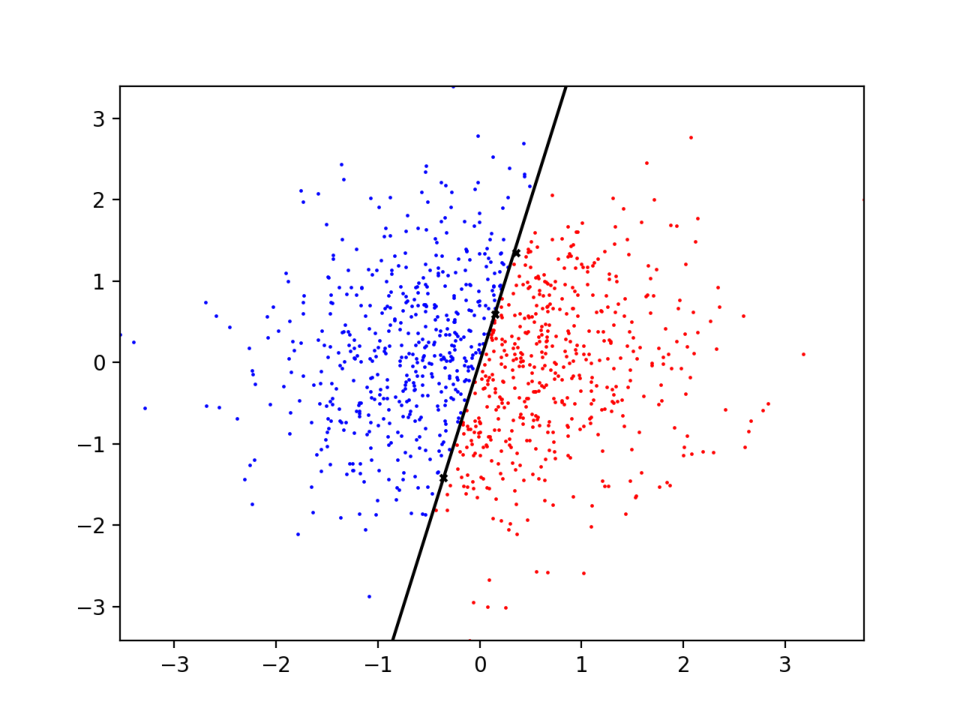
\includegraphics[width=0.5\textwidth]{fig/fig_linear_simplemodel_03err_train} & 
  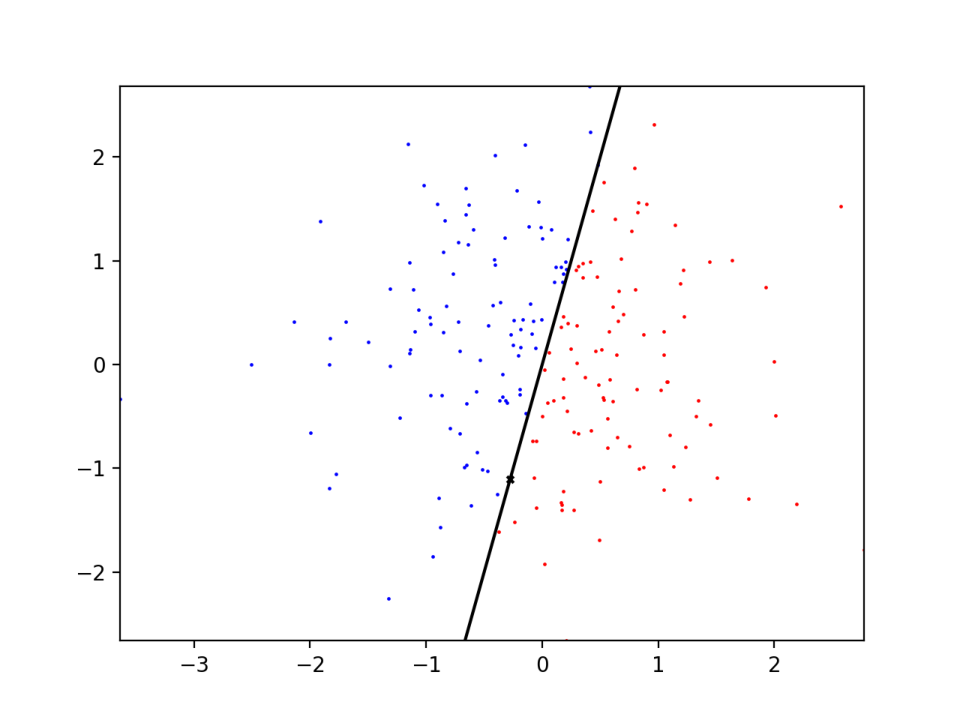
\includegraphics[width=0.5\textwidth]{fig/fig_linear_simplemodel_05err_test} \\
  \end{tabular}
   \caption{Training (left) and test (right) sets for the first simple model. 
   The discriminant between the two classes is a line, points belonging to class 0 and 1 are marked in blue and red, respectively. 
   Points misclassified are marked with a black x symbol.  \label{fig_lin_results}}
  \end{center}
  \end{figure}
  % End of fig2
  
For this problem and all the following once we sampled 1000 points in the train set and 200 points in test set. 
The learning rate is set equal to $0.05$ for all problems and we run it for 1000 epochs. 

As one could have expected, this very simple linear model does not generalise to more complex classification problems, where there discriminant plane is non linear, as  for example the dataset required for this project. 
After  randomly generating points  in $[0,1]^2$  (sampled from a uniform distribution) with label 0 if they lie inside the circle of radius $\frac{1}{\sqrt{2 \pi}}$ or 1 otherwise, we test the classifier using  the simple linear model presented above.
Figure \ref{fig_circle_simple} shows the results on an unseen test set.
All the points close to circle, the discriminant border, are misclassified (black cross) leading to an error of 10.2\% in the training set and 11\% in the test set. 
 %Fig2
  \begin{figure}[h]
 \begin{center}
\begin{tabular}{l r}
  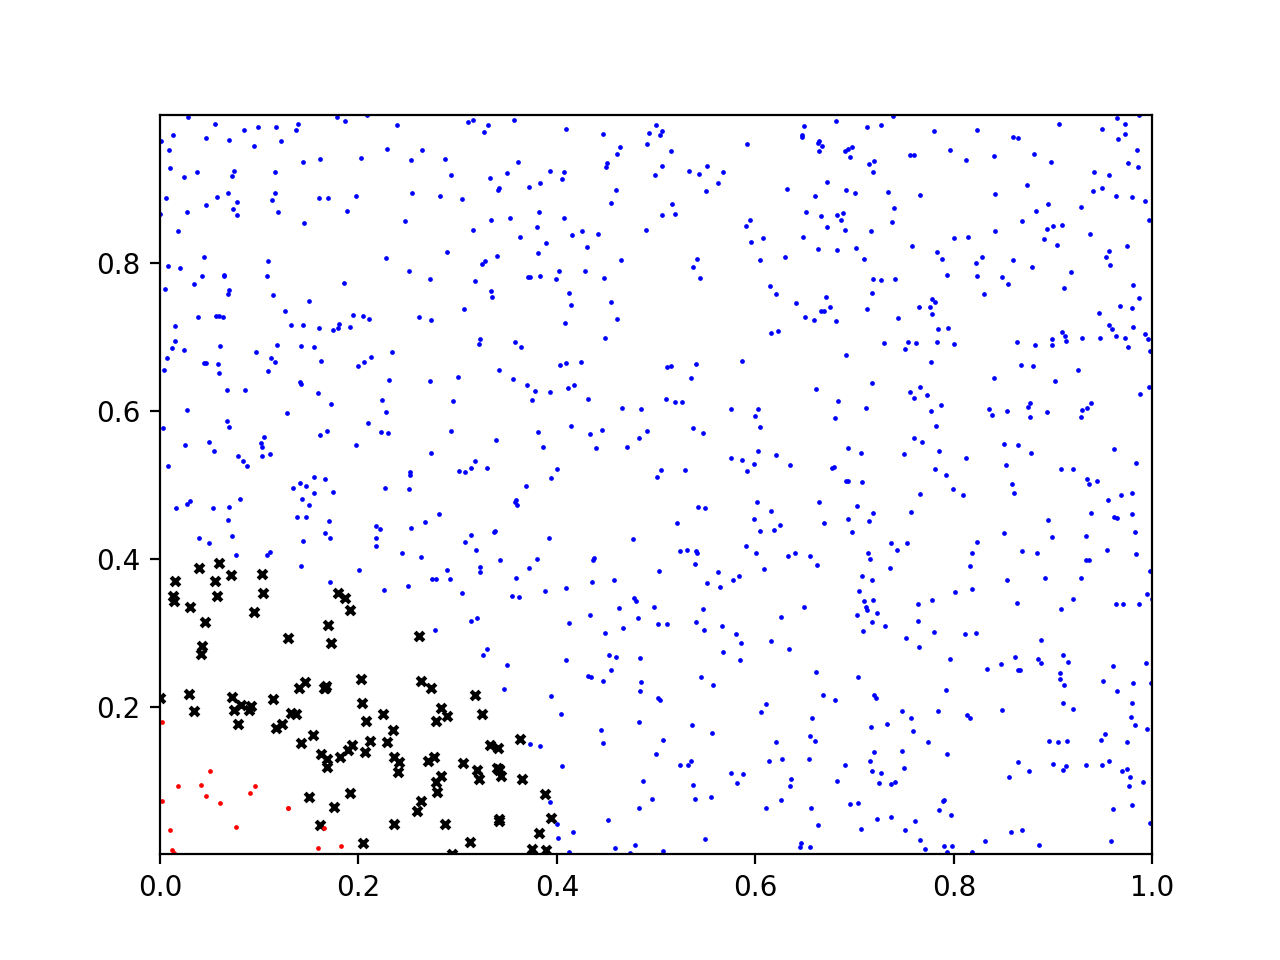
\includegraphics[width=0.5\textwidth]{fig/fig_circ_simplemodel_102err_train} & 
  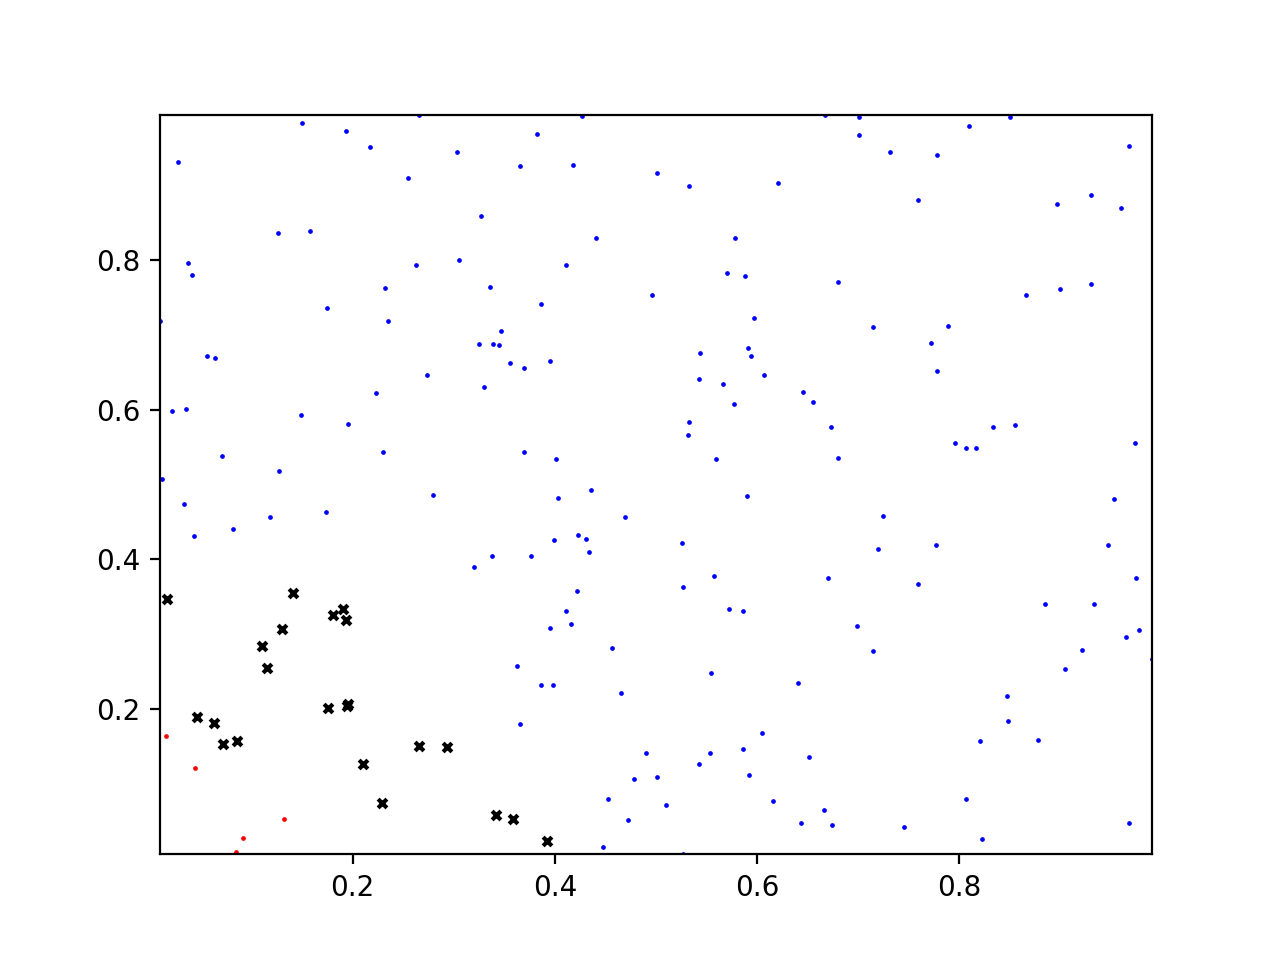
\includegraphics[width=0.5\textwidth]{fig/fig_circ_simplemodel_11err_test} \\
  \end{tabular}
   \caption{Training (left) and test (right) sets for the first simple model on the requested data. The discriminant between the two classes is a circle, points belonging to class 0 and 1 are marked in blue and red, respectively. Points misclassified are marked with a black x symbol.  \label{fig_circle_simple}}
  \end{center}
  \end{figure}
  % End of fig2
  
It seems evident that for this setup a network with more capacity and nonlinear activation functions is needed to increase the accuracy.
After this preliminary set, we are ready to test the performance of  the model described in the assignement, characterized by 3 hidden layers of dimension 25. See Figure \ref{fig_circle_good} for qualitatively results on training and test sets.
Here we obtain 0.5\% error on the training set and 0\% error on the test set.
These results are very satisfying and confirm the well behaviour of the model we implemented. 
   %Fig3
  \begin{figure}[h]
 \begin{center}
\begin{tabular}{l r}
  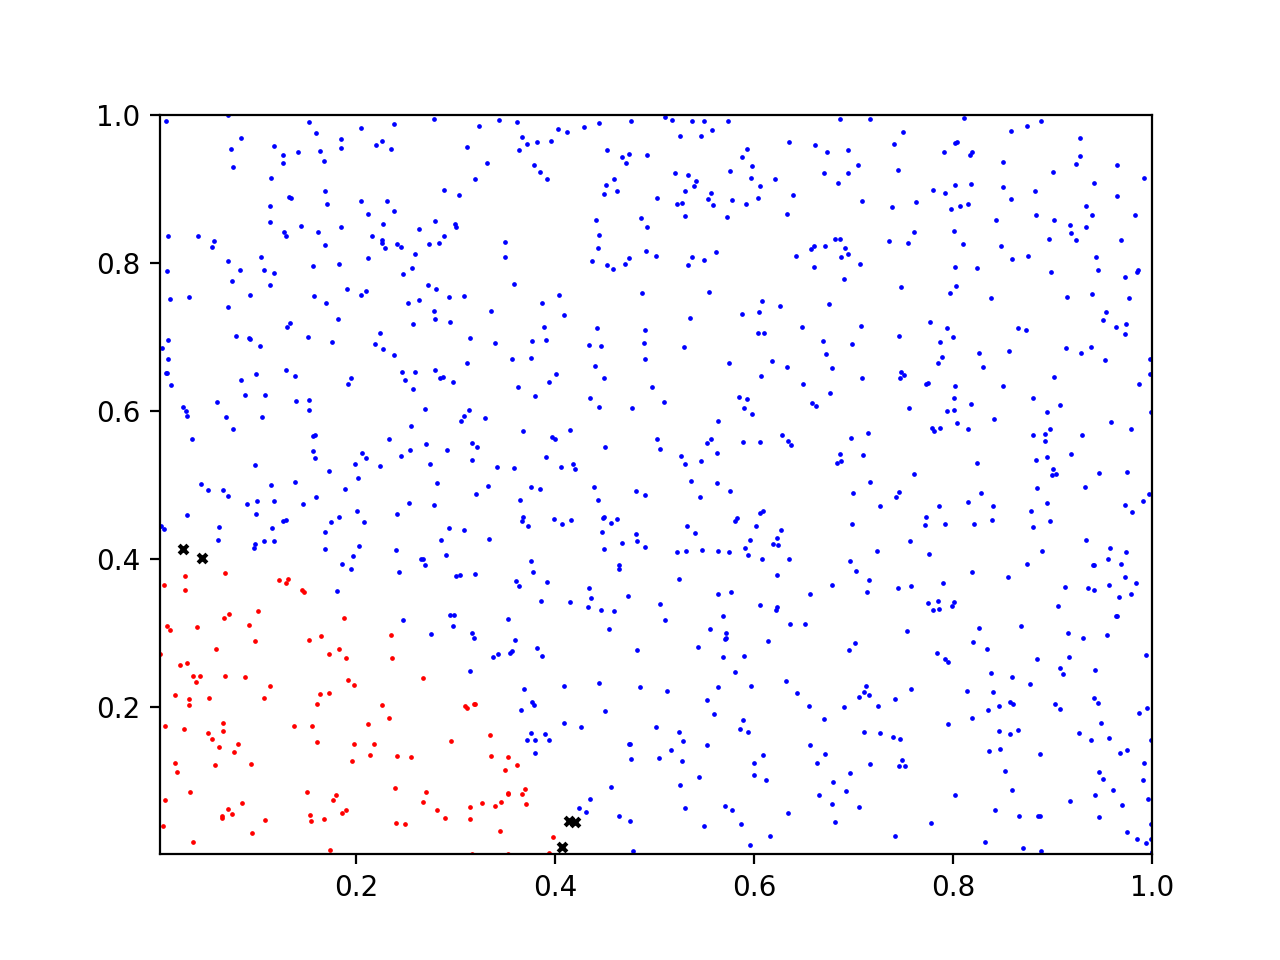
\includegraphics[width=0.5\textwidth]{fig/fig_circ_ourmodel_05err_train} & 
  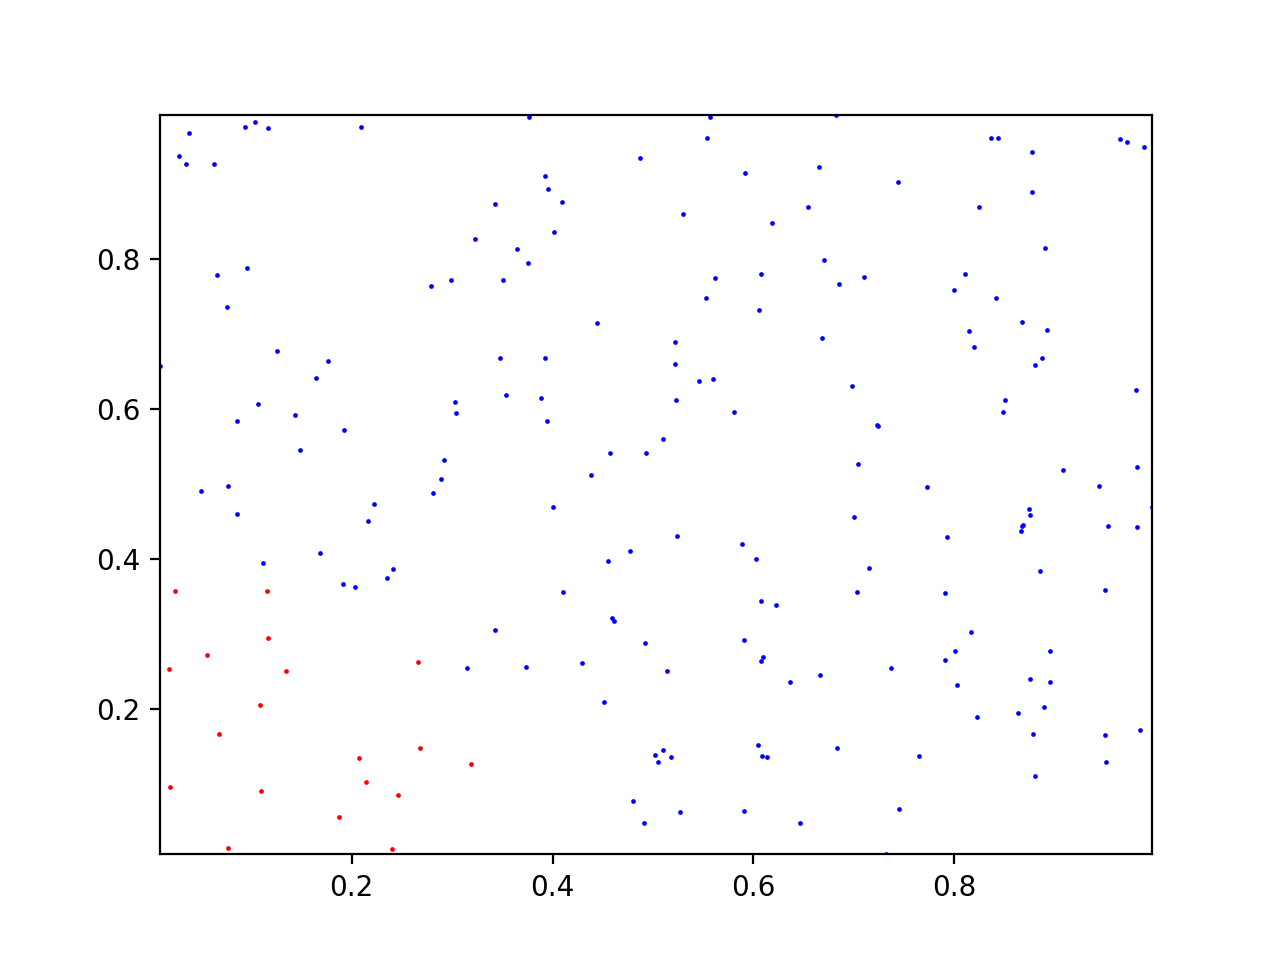
\includegraphics[width=0.5\textwidth]{fig/fig_circ_ourmodel_0err_test} \\
  \end{tabular}
   \caption{Training (left) and test (right) sets for the non-linear discriminant problem using the model described in Section \ref{sec_code}. Points belonging to class 0 and 1 are marked in blue and red, respectively and  points which are misclassified are marked with a black x symbol.  \label{fig_circle_good}}
  \end{center}
  \end{figure}
  % End of fig3

% Conclusion
 \section{Conclusion}\label{sec_conclusion}
We developed a framework for Neural Network and tested it on different toy problems. The interface of the code, in particular the design of the network, is easy to understand from the user point of view and permits several different configurations with minor changes with respect to the test case. Even though the structure of the code allows only "converging" graph, and not general acyclic structure, the possibilities offered by our approach go beyond simple sequential networks.
Standard nonlinear activation functions have been tested, showing results that are in accordance with the expected ones. Simple networks seems to give an accurate solution for trivial classification problems while more articulate and long structures seem necessary as the complexity grows.
 
 % References
\bibliographystyle{abbrv}
\bibliography{mybib_dl} 
  
  
  
\end{document}